% Provenance (never printed): see sources/outline_sources.md (Year 2: ancient massifs,
% Caledonian and Variscan belts; the Wilson cycle; supercontinents). Caledonian phases after
% McKerrow, Mac Niocaill and Dewey (2000) and Schiffer et al. (2020); the Wilson cycle after
% Chenin et al. (2018) and Schiffer et al. (2020); the Variscan belt after Faure (2024);
% supercontinents after Nance (2022); Siccar Point after the IUGS Geoheritage description.
% Model ocean and supercontinent chart from figdata/bachelor-2/wilson.py. Exercise and problem
% values in the Book 4 scratch calculator calc/ch15.py.
\chapter{Ancient Massifs and the Wilson Cycle}\label{ch:b2:wilson-cycle}

On the coast of south-east Scotland, at Siccar Point, grey beds of sandstone stand on end
under a cap of red sandstone that dips gently towards the sea. The grey beds were laid down in
an ocean early in the Silurian, then folded and cleaved when that ocean closed; they were worn
down to an uneven surface; in the Late Devonian red gravels buried them, and a second,
gentler mountain building tilted the red beds in turn. One cliff records an ocean that has
vanished, a mountain belt that has gone, and the next one. This chapter reads such records,
gathers them into a cycle that ocean basins follow, and steps back to the longest rhythm of
all, the assembly and break-up of \omterm{def:b2:wilson-cycle:supercontinent}{supercontinents}.
% ledger: iugs:siccar-orogenies, iugs:siccar-point

\begin{recall}
\textbf{From the school volumes}: Pangaea and its break-up, \omterm{def:b2:wilson-cycle:supercontinent}{supercontinents}; unconformities;
the denudation rate, isostatic rebound, and the exponential decay of a mountain range worn
down by its rivers. \textbf{From the Year 1 volume}: continental rifts, passive margins and
mid-ocean ridges, the full and half spreading rates; subduction and active margins.
\textbf{From \cref{ch:b2:crustal-melting} to \cref{ch:b2:himalaya-andes}}: \omterm{def:b2:crustal-melting:migmatite}{migmatites} and
granites; \omterm{def:b2:alpine-orogen:orogen}{orogen}, \omterm{def:b2:alpine-orogen:ophiolite}{ophiolite}, suture, \omterm{def:b2:alpine-orogen:nappes}{nappe}, \omterm{def:b2:alpine-orogen:foreland}{flysch} and \omterm{def:b2:alpine-orogen:foreland}{molasse}, \omterm{def:b2:alpine-orogen:foreland}{foreland basin}; collision and
\omterm{def:b2:himalaya-andes:types}{Andean-type orogens}; \omterm{def:b2:himalaya-andes:thickening}{crustal thickening}, Airy thickness and \omterm{def:b2:himalaya-andes:collapse}{gravitational collapse}.
\end{recall}

\begin{omfigure}
\centering
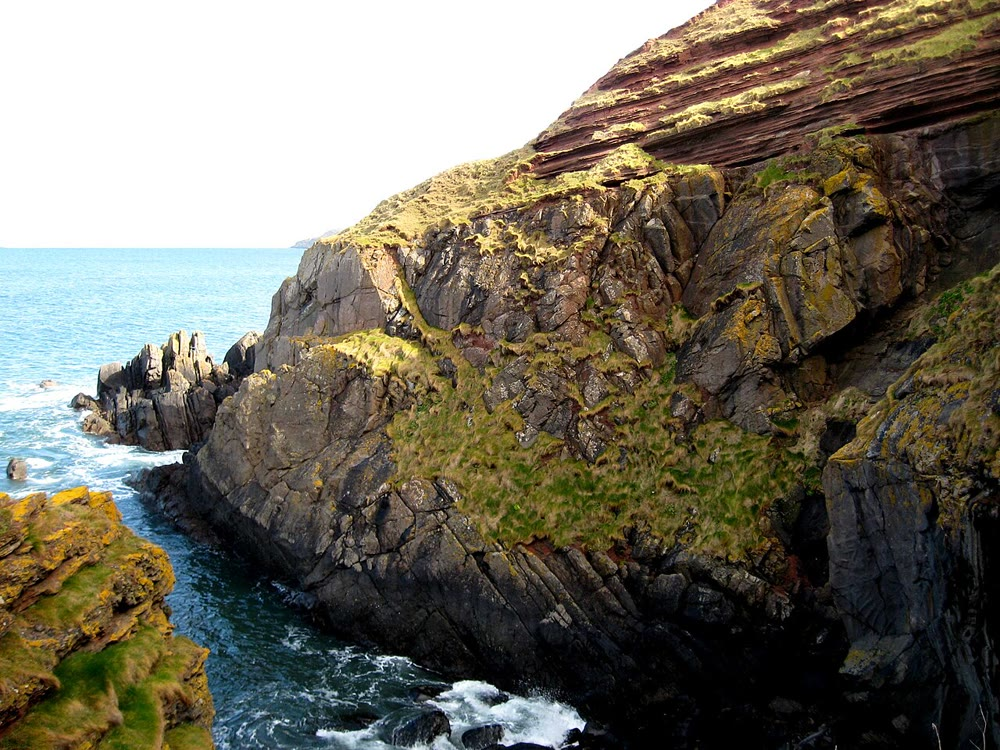
\includegraphics[width=0.64\linewidth]{images/book4/b2-15-siccar-point.jpg}
\par\smallskip{\small Siccar Point, south-east of the point: near-vertical beds of grey
Silurian greywacke, folded in the Caledonian orogeny, under gently dipping red beds of the
Upper Devonian. Photograph dave souza, 2008, CC BY-SA 4.0.}
\end{omfigure}
% ledger: iugs:siccar-orogenies

\section{Belts worn to their roots}\label{sec:b2:wilson-cycle:old}

Western Europe and eastern North America are crossed by mountain belts far older than the
Alps. Their summits have gone, but their rocks remain. Three of them matter here.

The \emph{Caledonian} belt runs from Norway through Scotland and Ireland to Newfoundland and
the northern Appalachians, and on through East Greenland and Svalbard. It is the record of an
ocean, the Iapetus, that lay in the early Palaeozoic between Laurentia, the ancestor of North
America and Greenland, to the north-west, and Baltica and Avalonia to the south-east and east.
Its margins had rifted about 600 million years ago; its closure, from the Cambrian to the
Devonian, produced a whole series of collisions, so that the Caledonian orogeny spans some
200 million years. The term names a place and an ocean, not an age.
% ledger: mckerrow00:caledonian, schiffer20:caledonides

The \emph{Variscan} belt, called Hercynian in older texts, crosses Europe from south-west
England and Belgium through France and Iberia into central Europe; the \emph{Appalachian} belt of
eastern North America is its western twin. Together they record the closure of the oceans
between the southern continent, Gondwana, and the northern one, which had just been welded by
the Caledonian collisions. Their last collision, in the Late Carboniferous and Permian, left
a fold belt running east--west through southern Europe and north-east--south-west between
eastern North America and north-west Africa, and with it the \omterm{def:b2:wilson-cycle:supercontinent}{supercontinent} Pangaea.
% ledger: schiffer20:variscan, faure24:variscan

How does one recognise a mountain belt that has been eroded for three hundred million years?
Not by its relief, which has gone. One looks for its parts, each of which the previous
chapters have met:
\begin{itemize}
\item \emph{sutures} lined with \emph{\omterm{def:b2:alpine-orogen:ophiolite}{ophiolites}}, slices of the ocean floor that closed;
\item belts of \emph{metamorphic rocks}, often of high grade, the roots of the thickened crust,
now at the surface because the kilometres above them were eroded;
\item \emph{granites} and \emph{\omterm{def:b2:crustal-melting:migmatite}{migmatites}}, the products of the crustal melting that
thickening and heating bring;
\item sediments of the closing ocean and of the belt: \emph{\omterm{def:b2:alpine-orogen:foreland}{flysch}} shed into deep basins
during the convergence, \emph{\omterm{def:b2:alpine-orogen:foreland}{molasse}} shed into foreland and intramontane basins;
\item \emph{angular unconformities}, where younger beds rest on beds that were folded and
eroded before them, dating the deformation between the two.
\end{itemize}

\begin{definition}[Peneplain]\label{def:b2:wilson-cycle:peneplain}
A \emph{peneplain}\index{peneplain} is a land surface of low relief, near the base level of
erosion, cut across rocks of different hardness and structure by long erosion of a former
relief.
\end{definition}

The Variscan belt is a hot \omterm{def:b2:alpine-orogen:orogen}{orogen}. In the Alps of \cref{ch:b2:alpine-orogen}, the rocks
followed metamorphic gradients of about \qty{8}{\celsius} per kilometre; in the Variscan belt,
about \qty{30}{\celsius} per kilometre. Its crust melted widely: in the French Massif Central
and Armorican Massif, \omterm{def:b2:crustal-melting:migmatite}{migmatites} formed between about 330 and 325 million years ago, and
granites intruded them. That melting is the main difference from the Western Alps. As the
collision ended, the thickened crust thinned by extension, metamorphic rocks were brought up
along detachments, and intramontane basins opened; then erosion levelled the chain into a
Permian and Triassic \omterm{def:b2:wilson-cycle:peneplain}{peneplain} on which the sediments of the next cycle were laid.
% ledger: faure24:variscan

\begin{omfigure}
\centering\small
\begin{tabular}{>{\raggedright\arraybackslash}p{0.2\linewidth}|>{\raggedright\arraybackslash}p{0.17\linewidth}|>{\raggedright\arraybackslash}p{0.52\linewidth}}
phase & age & what collided \\ \hline
Penobscotian & 490--485 Ma & an island arc thrust onto the Avalonian margin \\
Grampian, Taconian & 480--455 Ma & island arcs against Laurentia (Scotland; the northern Appalachians) \\
Shelveian & early Late Ordovician & Avalonia against Baltica; the Tornquist Sea closes \\
Scandian & 425--400 Ma & Baltica against Laurentia; the great \omterm{def:b2:alpine-orogen:nappes}{nappes} of Scandinavia \\
Acadian & Early Devonian & \omterm{def:b2:wilson-cycle:terrane}{terranes} from Gondwana against the new continent; Iapetus closed \\
\end{tabular}
\par\smallskip{\small The main phases of the Caledonian orogeny. The early phases are
collisions of arcs with arcs or continents, the late ones collisions of continents; most
phases began at different times in different places.}
\end{omfigure}
% ledger: mckerrow00:phases, schiffer20:caledonides

The Caledonian table above shows the other mark of old belts: they are composite. Before the
two continents met, arcs and smaller blocks came in one by one and were welded on.

\begin{definition}[Terrane; microcontinent]\label{def:b2:wilson-cycle:terrane}
A \emph{terrane}\index{terrane} is a fault-bounded block of crust whose geological history
differs from that of its neighbours, brought to its present position by plate motion; it may
be an island arc, an oceanic plateau, a slice of ocean floor or a fragment of continent. A
\emph{microcontinent}\index{microcontinent} is a block of continental crust, smaller than a
continent, separated from the continents by oceanic crust.
\end{definition}

Avalonia was such a block: a strip of crust that left the margin of Gondwana, opened the Rheic
Ocean behind it in the Ordovician, crossed the Iapetus and docked against Baltica and then
Laurentia. Armorica and Saxothuringia, now in France and Germany, followed it in turn; their
sutures, marked by \omterm{def:b2:alpine-orogen:ophiolite}{ophiolites}, divide the Variscan belt into zones from a northern foreland
in the old northern continent to a southern foreland in Gondwana.
% ledger: schiffer20:caledonides, schiffer20:variscan, faure24:variscan

\begin{omfigure}
\centering
\begin{tikzpicture}[x=0.5cm, y=0.5cm, font=\scriptsize]
\tikzset{cont/.style={fill=orange!25, draw=black!60, line width=0.4pt},
  terr/.style={fill=orange!45, draw=black!60, line width=0.4pt},
  ocn/.style={font=\scriptsize\itshape, text=blue!50!black},
  belt/.style={pattern=north east lines, pattern color=red!60!black, draw=red!60!black}}
% panel A
\begin{scope}
\fill[blue!6] (0,0) rectangle (9,8);
\draw[cont] (0.3,4.2) -- (3.0,4.0) -- (3.4,7.7) -- (0.3,7.7) -- cycle;
\node[align=center] at (1.7,6.0) {Lau-\\rentia};
\draw[cont] (6.0,5.4) -- (8.7,5.0) -- (8.7,7.7) -- (6.4,7.7) -- cycle;
\node at (7.4,6.6) {Baltica};
\draw[cont] (0.3,0.3) -- (8.7,0.3) -- (8.7,1.6) -- (0.3,1.9) -- cycle;
\node at (4.5,0.95) {Gondwana};
\draw[terr] (3.8,2.4) -- (6.6,2.2) -- (6.6,2.9) -- (3.8,3.1) -- cycle;
\node at (5.2,2.65) {Avalonia};
\node[ocn] at (4.6,5.4) {Iapetus};
\node[ocn] at (7.7,2.55) {Rheic};
\node[anchor=north west, font=\small\bfseries] at (0.1,8.9) {A: about 480 Ma};
\end{scope}
% panel B
\begin{scope}[xshift=5.0cm]
\fill[blue!6] (0,0) rectangle (9,8);
\draw[cont] (0.3,3.6) -- (3.0,3.4) -- (3.4,7.7) -- (0.3,7.7) -- cycle;
\draw[cont] (3.0,3.4) -- (3.4,7.7) -- (8.7,7.7) -- (8.7,4.4) -- (5.2,4.6) -- (5.0,3.4) -- cycle;
\draw[terr] (3.0,3.4) -- (5.0,3.4) -- (5.2,4.6) -- (8.7,4.4) -- (8.7,3.6) -- (3.0,2.8) -- cycle;
\draw[red!60!black, line width=1.2pt] (3.0,3.4) -- (3.4,7.7);
\draw[red!60!black, line width=1.2pt] (5.0,3.4) -- (5.2,4.6) -- (8.7,4.4);
\node[align=center] at (1.6,5.6) {Lau-\\rentia};
\node at (6.6,5.7) {Baltica};
\node at (6.4,3.75) {Avalonia};
\node at (6.0,7.1) {\textbf{Laurussia}};
\draw[cont] (0.3,0.3) -- (8.7,0.3) -- (8.7,1.3) -- (0.3,1.5) -- cycle;
\node at (4.5,0.8) {Gondwana};
\draw[terr] (2.2,1.9) -- (3.6,1.9) -- (3.6,2.3) -- (2.2,2.3) -- cycle;
\draw[terr] (5.0,1.8) -- (6.6,1.8) -- (6.6,2.2) -- (5.0,2.2) -- cycle;
\node[ocn] at (7.7,2.3) {Rheic};
\node[anchor=north west, font=\small\bfseries] at (0.1,8.9) {B: about 420 Ma};
\end{scope}
% panel C
\begin{scope}[xshift=10.0cm]
\fill[blue!6] (0,0) rectangle (9,8);
\draw[cont] (0.3,3.0) -- (8.7,3.0) -- (8.7,7.7) -- (0.3,7.7) -- cycle;
\draw[cont] (0.3,0.3) -- (8.7,0.3) -- (8.7,3.0) -- (0.3,3.0) -- cycle;
\fill[belt] (0.3,2.5) -- (8.7,2.5) -- (8.7,3.5) -- (0.3,3.5) -- cycle;
\node[fill=orange!25, inner sep=1pt] at (4.5,5.6) {Laurussia};
\node[fill=orange!25, inner sep=1pt] at (4.5,1.3) {Gondwana};
\node[fill=white, fill opacity=0.85, text opacity=1, inner sep=1pt, align=center] at (4.5,3.0)
  {Variscan--Appalachian belt};
\node[ocn] at (7.6,0.7) {};
\node[anchor=north west, font=\small\bfseries] at (0.1,8.9) {C: about 300 Ma, Pangaea};
\end{scope}
\end{tikzpicture}
\par\smallskip{\small Three moments of the closure of the Iapetus and Rheic oceans, as a
schematic sketch with no map projection and no scale: positions, sizes and shapes are only
topological. A: Avalonia has left Gondwana and the Rheic Ocean opens behind it. B: Iapetus has
closed; Laurentia, Baltica and Avalonia form Laurussia, along Caledonian sutures (red lines);
smaller blocks are crossing the Rheic Ocean. C: Gondwana has met Laurussia along the
Variscan--Appalachian belt (hatched).}
\end{omfigure}
% ledger: mckerrow00:caledonian, mckerrow00:phases, schiffer20:caledonides, schiffer20:variscan, faure24:variscan

\section{The Wilson cycle}\label{sec:b2:wilson-cycle:cycle}

In 1966 J. Tuzo Wilson asked whether the Atlantic had closed and then
opened again. Fossils of the early and middle Palaeozoic told him that a wide ocean had then
separated the faunas of North America from those of Western Europe, an ocean that no longer
existed from the late Palaeozoic to the middle of the Mesozoic. The modern Atlantic had opened
nearly where that older ocean, the Iapetus, had closed.
% ledger: schiffer20:wilson, chenin18:cycle

\begin{definition}[Wilson cycle]\label{def:b2:wilson-cycle:wilson}
The \emph{Wilson cycle}\index{Wilson cycle} is the succession of stages through which an
ocean basin opens and closes again between continental margins: continental rifting,
break-up and sea-floor spreading, a widening ocean with passive margins, the start of
subduction, the narrowing and closure of the ocean, continental collision, and the collapse
and erosion of the belt, after which the welded continent may rift again along the same zone.
\end{definition}

The figure below follows the stages. They are those of the previous chapters put in order:
the rifts and passive margins of the Year 1 volume, the active margins and their arcs, the
Alpine and Himalayan collisions, the \omterm{def:b2:himalaya-andes:collapse}{gravitational collapse} of Tibet, the slow wearing-down
of the old belts.

\begin{omfigure}
\centering
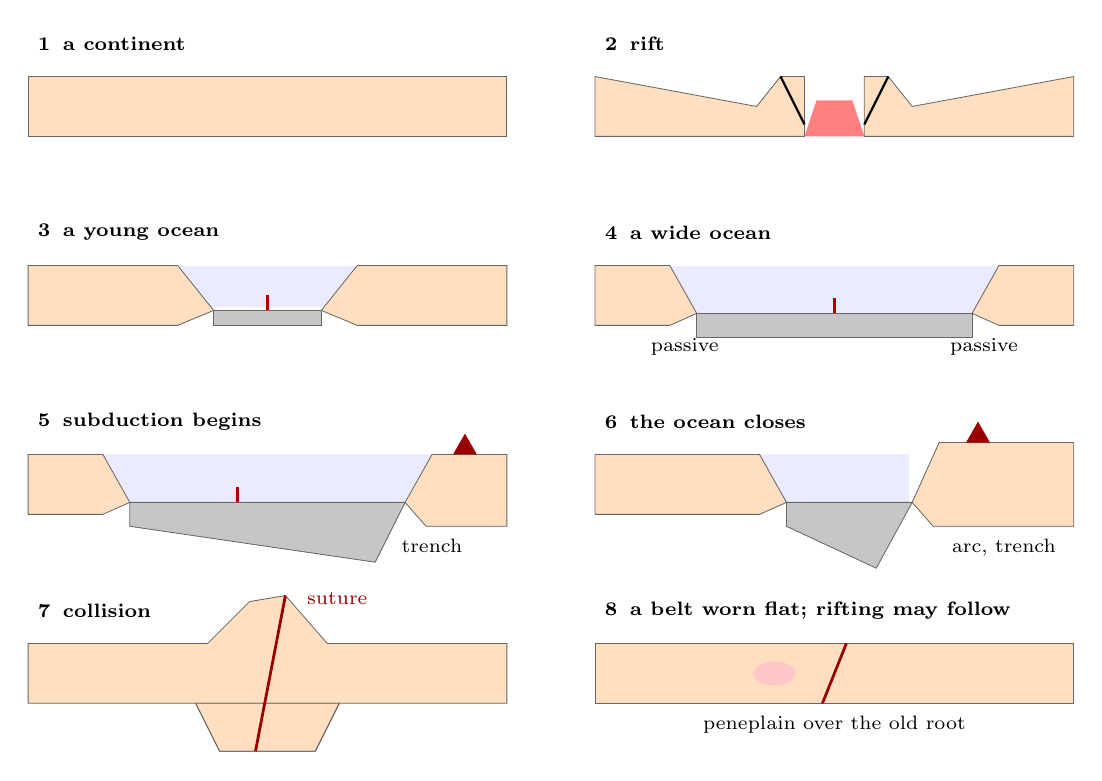
\begin{tikzpicture}[x=0.38cm, y=0.38cm, font=\scriptsize]
\tikzset{crust/.style={fill=orange!25, draw=black!60, line width=0.3pt},
  ocrust/.style={fill=gray!45, draw=black!60, line width=0.3pt},
  sea/.style={fill=blue!8},
  ttl/.style={anchor=west, font=\scriptsize\bfseries}}
% 1 continent
\begin{scope}
\draw[crust] (0,0) -- (16,0) -- (16,2) -- (0,2) -- cycle;
\node[ttl] at (0,3.1) {1\enspace a continent};
\end{scope}
% 2 rift
\begin{scope}[xshift=7.2cm]
\draw[crust] (0,0) -- (7,0) -- (7,2) -- (6.2,2) -- (5.4,1.0) -- (0,2) -- cycle;
\draw[crust] (9,0) -- (16,0) -- (16,2) -- (10.6,1.0) -- (9.8,2) -- (9,2) -- cycle;
\fill[red!50] (7,0) -- (9,0) -- (8.6,1.2) -- (7.4,1.2) -- cycle;
\draw[thick] (6.2,2) -- (7,0.4); \draw[thick] (9.8,2) -- (9,0.4);
\node[ttl] at (0,3.1) {2\enspace rift};
\end{scope}
% 3 young ocean
\begin{scope}[yshift=-2.4cm]
\fill[sea] (5,2) -- (11,2) -- (11,0.6) -- (5,0.6) -- cycle;
\draw[crust] (0,0) -- (5,0) -- (6.2,0.5) -- (5,2) -- (0,2) -- cycle;
\draw[crust] (16,0) -- (11,0) -- (9.8,0.5) -- (11,2) -- (16,2) -- cycle;
\draw[ocrust] (6.2,0.5) -- (9.8,0.5) -- (9.8,0) -- (6.2,0) -- cycle;
\draw[red!70!black, thick] (8,0.5) -- (8,1.0);
\node[ttl] at (0,3.1) {3\enspace a young ocean};
\end{scope}
% 4 wide ocean
\begin{scope}[xshift=7.2cm, yshift=-2.4cm]
\fill[sea] (2.5,2) -- (13.5,2) -- (13.5,0.4) -- (2.5,0.4) -- cycle;
\draw[crust] (0,0) -- (2.5,0) -- (3.4,0.4) -- (2.5,2) -- (0,2) -- cycle;
\draw[crust] (16,0) -- (13.5,0) -- (12.6,0.4) -- (13.5,2) -- (16,2) -- cycle;
\draw[ocrust] (3.4,0.4) -- (12.6,0.4) -- (12.6,-0.4) -- (3.4,-0.4) -- cycle;
\draw[red!70!black, thick] (8,0.4) -- (8,0.9);
\node[anchor=north] at (3,-0.1) {passive};
\node[anchor=north] at (13,-0.1) {passive};
\node[ttl] at (0,3.1) {4\enspace a wide ocean};
\end{scope}
% 5 subduction begins
\begin{scope}[yshift=-4.8cm]
\fill[sea] (2.5,2) -- (13.5,2) -- (13.5,0.4) -- (2.5,0.4) -- cycle;
\draw[crust] (0,0) -- (2.5,0) -- (3.4,0.4) -- (2.5,2) -- (0,2) -- cycle;
\draw[crust] (16,-0.4) -- (13.3,-0.4) -- (12.6,0.4) -- (13.5,2) -- (16,2) -- cycle;
\draw[ocrust] (3.4,0.4) -- (12.6,0.4) -- (11.6,-1.6) -- (3.4,-0.4) -- cycle;
\fill[red!60!black] (14.2,2) -- (14.6,2.7) -- (15.0,2) -- cycle;
\draw[red!70!black, thick] (7,0.4) -- (7,0.9);
\node[anchor=north] at (13.5,-0.5) {trench};
\node[ttl] at (0,3.1) {5\enspace subduction begins};
\end{scope}
% 6 ocean closes
\begin{scope}[xshift=7.2cm, yshift=-4.8cm]
\fill[sea] (5.5,2) -- (10.5,2) -- (10.5,0.4) -- (5.5,0.4) -- cycle;
\draw[crust] (0,0) -- (5.5,0) -- (6.4,0.4) -- (5.5,2) -- (0,2) -- cycle;
\draw[crust] (16,-0.4) -- (11.3,-0.4) -- (10.6,0.4) -- (11.5,2.4) -- (16,2.4) -- cycle;
\draw[ocrust] (6.4,0.4) -- (10.6,0.4) -- (9.4,-1.8) -- (6.4,-0.4) -- cycle;
\fill[red!60!black] (12.4,2.4) -- (12.8,3.1) -- (13.2,2.4) -- cycle;
\node[anchor=north west] at (11.6,-0.5) {arc, trench};
\node[ttl] at (0,3.1) {6\enspace the ocean closes};
\end{scope}
% 7 collision
\begin{scope}[yshift=-7.2cm]
\draw[crust] (0,0) -- (16,0) -- (16,2) -- (10,2) -- (8.6,3.6) -- (7.4,3.4) -- (6,2) -- (0,2) -- cycle;
\fill[crust] (5.6,0) -- (10.4,0) -- (9.6,-1.6) -- (6.4,-1.6) -- cycle;
\draw[black!60, line width=0.3pt] (5.6,0) -- (6.4,-1.6) -- (9.6,-1.6) -- (10.4,0);
\draw[red!60!black, line width=1pt] (8.6,3.6) -- (7.6,-1.6);
\node[anchor=west, text=red!60!black] at (9.0,3.5) {suture};
\node[ttl] at (0,3.1) {7\enspace collision};
\end{scope}
% 8 worn flat
\begin{scope}[xshift=7.2cm, yshift=-7.2cm]
\draw[crust] (0,0) -- (16,0) -- (16,2) -- (0,2) -- cycle;
\draw[red!60!black, line width=1pt] (8.4,2) -- (7.6,0);
\fill[pink!60!red!40] (6.0,1.0) ellipse (0.7 and 0.4);
\node[anchor=north] at (8,-0.1) {peneplain over the old root};
\node[ttl] at (0,3.1) {8\enspace a belt worn flat; rifting may follow};
\end{scope}
\end{tikzpicture}
\par\smallskip{\small The stages of the \omterm{def:b2:wilson-cycle:wilson}{Wilson cycle}, as schematic sections (not to scale):
continental crust in orange, oceanic crust in grey, the ridge in red, volcanoes of the arc as
triangles; in the last panel the suture and a granite remain in a crust of normal thickness.}
\end{omfigure}
% ledger: chenin18:cycle, schiffer20:wilson

\subsection{How wide, how long?}

An ocean grows by sea-floor spreading at its ridge and shrinks by subduction at its trenches.
Simple bookkeeping gives its width.

\begin{proposition}[Width of an ocean through a cycle]\label{prop:b2:wilson-cycle:width}
Let an ocean open at time $t_0$ and widen at the full spreading rate $V_s$ of its ridge, until a
subduction zone starts at one margin at time $t_1$ and consumes ocean floor at the rate $V_c$
relative to that margin, with $V_c > V_s$, the ridge still spreading. Its width is
\[
  W(t) = V_s\,(t - t_0) \quad (t_0 \le t \le t_1), \qquad
  W(t) = V_s\,(t_1 - t_0) - (V_c - V_s)\,(t - t_1) \quad (t \ge t_1),
\]
greatest at $t_1$, and the ocean closes a time $V_s(t_1 - t_0)/(V_c - V_s)$ after subduction
begins. With symmetric spreading, the ridge moves towards the trench at $V_c - V_s/2$.
\end{proposition}

\begin{proof}
Hold the margin with the trench fixed. Before $t_1$ the two margins separate at the full
spreading rate $V_s$, so the width grows at $V_s$ from zero. After $t_1$ the plate between
trench and ridge moves towards the trench at $V_c$; the ridge adds $V_s$ to the distance
between that plate and the far plate, so the far margin moves towards the trench at $V_c - V_s$,
the rate at which the width decreases. The width reaches zero after $V_s(t_1 - t_0)/(V_c -
V_s)$. With symmetric spreading the ridge moves at the mean of the velocities of the plates on
either side, $(V_c + (V_c - V_s))/2 = V_c - V_s/2$.
\end{proof}

The figure below plays this bookkeeping for a model ocean of the Iapetus type: spreading from
\qty{570}{Ma} at \qty{30}{mm} a year, subduction from \qty{490}{Ma} consuming \qty{60}{mm} a
year. The rates are assumptions, round values of the size measured today in the oceans; the
real Iapetus was neither so simple nor so well known. The model ocean reaches \qty{2400}{km}
and closes at \qty{410}{Ma}, within the time span of the Scandian collision.
% values (wilson.py): max_width_km 2400, closure_Ma 410; ledger: mckerrow00:caledonian, schiffer20:caledonides

\begin{omfigure}
\centering
% figdata/bachelor-2/wilson.py part ocean (model values: assumptions)
\begin{tikzpicture}
\begin{axis}[width=0.8\linewidth, height=5.0cm, x dir=reverse, xmin=360, xmax=600, ymin=0,
  ymax=3300, ytick={0,1000,2000,3000}, xlabel={age (\unit{Ma})}, ylabel={width of the ocean (\unit{km})},
  tick label style={font=\scriptsize}, label style={font=\small}, xtick={600,560,...,360}]
\addplot[omThm, line width=1.2pt] table[x=t_Ma, y=width_km] {figdata/out/bachelor-2-wilson-ocean.dat};
\draw[dashed, black!50] (axis cs:490,0) -- (axis cs:490,2400);
\draw[dashed, black!50] (axis cs:570,0) -- (axis cs:570,2750);
\draw[dashed, black!50] (axis cs:410,0) -- (axis cs:410,2750);
\node[font=\scriptsize, anchor=south] at (axis cs:570,2750) {spreading begins};
\node[font=\scriptsize, anchor=south west] at (axis cs:488,2400) {subduction begins};
\node[font=\scriptsize, anchor=south] at (axis cs:410,2750) {collision};
\node[font=\scriptsize, anchor=west] at (axis cs:540,600) {opening at $V_s$};
\node[font=\scriptsize, anchor=south west, align=left] at (axis cs:446,1150) {closing\\at $V_c - V_s$};
\end{axis}
\end{tikzpicture}
\par\smallskip{\small Width of a model ocean through one \omterm{def:b2:wilson-cycle:wilson}{Wilson cycle}, from
\cref{prop:b2:wilson-cycle:width} with $V_s = \qty{30}{mm}$ a year from \qty{570}{Ma} and $V_c
= \qty{60}{mm}$ a year from \qty{490}{Ma}. Time runs from left to right.}
\end{omfigure}

\subsection{Opening where it closed}

Wilson's idea rests on a mechanical one: an old belt is a weak zone, and a continent that is
pulled apart tends to break along its weak zones rather than through its strong, stable
interior.

\begin{definition}[Structural reactivation]\label{def:b2:wilson-cycle:reactivation}
The \emph{structural reactivation}\index{structural reactivation} of a pre-existing structure
(a fault, a shear zone, a suture, a lithological contact) is the renewed concentration of
deformation along it, under a later stress field that may differ from the one that formed it.
\end{definition}

The North Atlantic is the test case, and it passes only in part. In the Central Atlantic the
young ocean follows the Appalachians closely. Between Scandinavia and Greenland the break-up
broadly follows the Caledonian belt. Further south it does not: the Iapetus suture still runs
through northern England and central Ireland, and the Atlantic opened west of it, leaving
pieces of Laurentia's old crust on Europe's north-western margin, around Rockall and Hatton.
Further north-west, the Labrador Sea and Baffin Bay cut straight across older cratons and
belts. Old structures guide later rifts, but not always: a weakness that has cooled for more
than 30 to 50 million years may have become strong, and a new rift may follow the deeper
fabric of the mantle rather than the crustal suture. The \omterm{def:b2:wilson-cycle:wilson}{Wilson cycle} is a guide, not a law.
% ledger: schiffer20:wilson, schiffer20:reactivation

Not every cycle opens a wide ocean. Many \omterm{def:b2:alpine-orogen:orogen}{orogens} close embryonic oceans, rifts that had barely
started spreading, less than about \qty{500}{km} wide: the Alps, the Pyrenees, most of the
Variscan belt of western Europe. Others close wide, mature oceans, as the Scandinavian
Caledonides did. The difference shows at the end. A belt that closed a wide ocean carried a
long-lived arc, which drained the mantle beneath of its fusible part; its collapse was poor in
\omterm{def:b2:magma-emplacement:magma}{magma}, as in the Caledonides. A belt that closed a narrow basin sits on \omterm{def:b2:mantle-melting:fertility}{fertile mantle}; its
collapse can be rich in \omterm{def:b2:magma-emplacement:magma}{magma}, as in the Variscan belt, where the Moho is now flat and the
lower crust layered, read as basalt underplated beneath the crust or as lower crust sheared
while hot. Within a few tens of millions of years the heat
anomalies of a belt fade; its structures remain.
% ledger: chenin18:cycle

\section{Supercontinents}\label{sec:b2:wilson-cycle:supercontinents}

\begin{definition}[Supercontinent; supercontinent cycle]\label{def:b2:wilson-cycle:supercontinent}
A \emph{supercontinent}\index{supercontinent} is a landmass that gathers most of the Earth's
continental crust into a single block. The \emph{supercontinent cycle}\index{supercontinent
cycle} is the episodic assembly of the continents into a supercontinent and its later
break-up, repeated through Earth's history.
\end{definition}

Pangaea, which Wegener reconstructed and the school volumes described, existed from about 325
to 200 million years ago. Earlier \omterm{def:b2:wilson-cycle:supercontinent}{supercontinents} have been proposed: Pannotia about 620 to
580 million years ago, whose existence is debated; Rodinia about 950 to 800 million years ago;
Nuna, also called Columbia, about 1.6 to 1.4 billion years ago; and, more doubtful, Kenorland
about 2.7 to 2.5 billion years ago and Ur about 3.0 billion years ago. They seem to have
assembled and broken up at intervals of roughly half a billion years since perhaps the late
Archaean. The cycle has been linked to the ages of mountain building, to peaks in the ages of
granites and of the zircon grains they contain, to the growth of the crust, to large igneous
provinces, to sea level and to climate: the assembly of a \omterm{def:b2:wilson-cycle:supercontinent}{supercontinent} tends to coincide
with cooling.
% ledger: nance22:supercontinents

\begin{omfigure}
\centering
% figdata/bachelor-2/wilson.py part supercontinents; ledger: nance22:supercontinents
\begin{tikzpicture}
\begin{axis}[width=0.86\linewidth, height=4.6cm, x dir=reverse, xmin=0, xmax=3300, ymin=-0.7,
  ymax=6.5, ytick=\empty, xlabel={age (\unit{Ma})}, tick label style={font=\scriptsize},
  label style={font=\small}, xtick={0,500,...,3000}, axis y line*=left,
  nodes near coords, point meta=explicit symbolic,
  nodes near coords style={font=\scriptsize, anchor=south, yshift=1pt}]
\addplot[only marks, mark=*, mark size=1.6pt, omThm,
  error bars/.cd, x dir=both, x explicit, error bar style={line width=3pt, omThm!60}, error mark=none]
  table[x=mid_Ma, y=row, x error=half_Ma, meta=name] {figdata/out/bachelor-2-wilson-supercontinents.dat};
\end{axis}
\end{tikzpicture}
\par\smallskip{\small \omterm{def:b2:wilson-cycle:supercontinent}{Supercontinents} through Earth's history, from assembly to break-up as
dated in a recent review: the bars span the quoted intervals (Ur is a single estimate), the
dots their midpoints. Pannotia, Kenorland and Ur are debated. Time runs from left to right.}
\end{omfigure}

Is the cycle truly periodic? The midpoints of the intervals in the chart are separated by 400,
1100, 625, 275 and 337.5 million years: on average about 550, but scattered by a factor of
four. ``Roughly half a billion years'' is a tendency, not a clock, and the earlier
\omterm{def:b2:wilson-cycle:supercontinent}{supercontinents} rest on sparse evidence.
% values (wilson.py): spacings 400 1100 625 275 337.5, mean 547.5 Myr

\section{From mountains to plains}\label{sec:b2:wilson-cycle:erosion}

What turns a belt like the Himalaya into the low hills of Brittany? The high-school volume
built a model: rivers wear a range down at a rate proportional to its mean elevation, $kh$,
and every metre removed from the top is partly given back by isostatic rebound, so that only
the fraction $f = (\rho_m - \rho_c)/\rho_m$ of it is lost as height. The mean elevation then
decays as
\[
  h(t) = h_0\,e^{-k f t} ,
\]
with the time constant $\tau = 1/(kf)$. In large mid-latitude basins, the denudation rate is
proportional to the mean relief, and without uplift the relief would fall to a tenth of its
value in about 11 million years: $k = \ln 10/11 \approx 0.21$ per million years. With the
densities 2700 and \qty{3300}{kg.m^{-3}}, $f = 0.18$ and $\tau \approx \qty{26}{Myr}$: a
range \qty{3}{km} high still stands \qty{1}{km} high some 30 million years later, and sinks
below \qty{300}{m} after about 60 million years.
% ledger: ahnert70:decay; values (wilson.py): k 0.20933 /Myr, f 0.18182, tau 26.275 Myr

The same rebound explains why old belts expose their roots. To bring a crust thickened from
$H$ to $T$ back to sea level, all the extra thickness $T - H$ must be eroded, while the mean
elevation was only $(T - H)f$: about 5.5 times more rock is removed than the height of the
range. Rocks that were 20 or \qty{30}{km} deep in the root come to the surface: the
\omterm{def:b2:crustal-melting:migmatite}{migmatites}, granites and high-grade gneisses of the old massifs, such as those of the Massif
Central.
% ledger: ahnert70:decay

The Variscan chain, whose last collisions ended about 290 million years ago, had been
levelled into a \omterm{def:b2:wilson-cycle:peneplain}{peneplain} during the Permian and Triassic: within the 60 million years or so
that the model gives. Collapse can make it faster: the extension of a thickened crust, as in
Tibet today, thins it directly, without waiting for the rivers. And at Siccar Point, Late Devonian gravels rest on
Silurian beds folded in the Caledonian collisions, on an old land surface that still keeps
some relief between the hard and the soft beds.
% ledger: faure24:variscan, iugs:siccar-orogenies

\begin{inthefield}[Reading an angular unconformity]
Geologists who study an angular unconformity such as Siccar Point begin by measuring the
attitude of the beds below and above the surface, strike and dip, at many places. They look
for the way up of the lower beds, by graded bedding or by the marks on the bases of the beds,
since folded beds can be overturned. They examine the surface itself: its relief, the
weathering beneath it, the pebbles of the older rocks in the conglomerate above it. Then they
date: the youngest fossils below give the age before which the folding cannot have happened,
the oldest fossils above the age before which it had happened and the land had been worn
down. The gap between the two brackets the orogeny. At Siccar Point the lower beds are early
Silurian and the upper ones Late Devonian, and the Caledonian folding, uplift and erosion fit
between; the gentle tilt of the upper beds is younger again, Variscan.
\end{inthefield}
% ledger: iugs:siccar-orogenies, ics:base.Silurian, ics:base.Devonian, ics:base.Carboniferous

\section*{Exercises}\label{sec:b2:wilson-cycle:exercises}

Data for the exercises: $g = \qty{9.8}{m.s^{-2}}$; densities of crust and mantle
\qty{2700}{kg.m^{-3}} and \qty{3300}{kg.m^{-3}}; normal crust $H = \qty{35}{km}$; ages of the
bases of the Silurian, Devonian and Carboniferous 443.1, 419.6 and \qty{358.9}{Ma}, of the
Triassic \qty{251.9}{Ma}.

\begin{exercise}[$\star$]\label{exo:b2:wilson-cycle:1}
The margins of the Iapetus rifted about \qty{600}{Ma}; the main Caledonian collision, the
Scandian, ended about \qty{400}{Ma}; the first arc--continent collision with Laurentia began
about \qty{480}{Ma}. (a) How long did the whole cycle of the Iapetus last? (b) How long did the
collisions last? (c) Why should ``Caledonian'' not be used to mean an age?
\end{exercise}

\begin{exercise}[$\star$]\label{exo:b2:wilson-cycle:2}
Put these situations in the order of the \omterm{def:b2:wilson-cycle:wilson}{Wilson cycle} and name the stage of each: (a) the
Red Sea, a narrow ocean between young rifted margins; (b) the Himalaya; (c) the East African
rift; (d) the Atlantic Ocean, wide, with passive margins on both sides; (e) the Pacific margin
of South America; (f) the low hills of Brittany on an old granite and gneiss basement.
\end{exercise}

\begin{exercise}[$\star$]\label{exo:b2:wilson-cycle:3}
At Siccar Point early Silurian beds lie under Late Devonian ones. (a) Between which bounds,
given by the data above, must the folding, uplift and erosion have taken place? (b) What is
the longest time they could have taken? (c) List in order the events the cliff records.
\end{exercise}

\begin{exercise}[$\star$]\label{exo:b2:wilson-cycle:4}
Say whether each is a \omterm{def:b2:wilson-cycle:terrane}{terrane}, a \omterm{def:b2:wilson-cycle:terrane}{microcontinent}, both or neither, and why: (a) Avalonia;
(b) Laurentia; (c) an island arc accreted to a continent; (d) the Iapetus suture.
\end{exercise}

\begin{exercise}[$\star\star$]\label{exo:b2:wilson-cycle:5}
Take the midpoints of the intervals of the \omterm{def:b2:wilson-cycle:supercontinent}{supercontinents} Ur (3000), Kenorland (2600),
Nuna (1500), Rodinia (875), Pannotia (600) and Pangaea (262.5), in millions of years ago.
(a) Compute the five spacings and their mean. (b) What is the ratio of the largest spacing to
the smallest? (c) Drop Kenorland and Ur, which are doubtful: what is the mean spacing of the
other four? Is ``half a billion years'' a period?
\end{exercise}

\begin{exercise}[$\star\star$]\label{exo:b2:wilson-cycle:6}
An ocean \qty{3000}{km} wide begins to be subducted at one margin at \qty{70}{mm} a year,
while its ridge spreads at \qty{25}{mm} a year. (a) How long does it take to close?
(b) How long if spreading stops at once? (c) Which plate's motion sets the closing rate after
the ridge has been subducted?
\end{exercise}

\begin{exercise}[$\star\star$]\label{exo:b2:wilson-cycle:7}
Suppose that crustal melting starts at about \qty{700}{\celsius} and that the surface is at
\qty{0}{\celsius}. (a) At what depth is that temperature reached along a gradient of
\qty{8}{\celsius} per kilometre? Of \qty{30}{\celsius} per kilometre? (b) Which belt, the
Alps or the Variscan belt, should then expose \omterm{def:b2:crustal-melting:migmatite}{migmatites} and granites of crustal origin?
(c) Why does a fixed gradient overstate the depth in the first case?
\end{exercise}

\begin{exercise}[$\star\star$]\label{exo:b2:wilson-cycle:8}
The Variscan collisions ended about \qty{290}{Ma}; a \omterm{def:b2:wilson-cycle:peneplain}{peneplain} had formed by the Permian and
Triassic. Use the decay model of the chapter, $\tau = \qty{26.3}{Myr}$. (a) How long does a
range take to fall from a mean elevation of \qty{3}{km} to \qty{0.3}{km}? (b) At what age would
that be? (c) What time constant would bring it there by the base of the Triassic? (d) What
process can shorten the time?
\end{exercise}

\begin{exercise}[$\star\star$]\label{exo:b2:wilson-cycle:9}
(a) Explain why the Iapetus suture in northern England and central Ireland, and Laurentian
crust near Rockall, show that the Atlantic did not reopen exactly along the old suture.
(b) What would a geologist expect to find in the old basement on either side of the suture
in Ireland? (c) The Appalachians had been deformed until the Early Permian; rifting began
about 80 million years after the orogeny. Compare with the 30 to 50 million years after which
a cooled zone may be too strong to reactivate.
\end{exercise}

\begin{exercise}[$\star\star\star$]\label{exo:b2:wilson-cycle:10}
An ocean \qty{3000}{km} wide has its ridge in the middle, \qty{1500}{km} from a trench that
consumes the plate on its side at \qty{70}{mm} a year; the ridge spreads at \qty{40}{mm} a
year, symmetrically. (a) How fast does the ridge approach the trench? (b) When does it reach
it? (c) How wide is the ocean then? (d) What happens to the volcanic arc when a ridge is
subducted?
\end{exercise}

\begin{exercise}[$\star\star\star$]\label{exo:b2:wilson-cycle:11}
A collision thickens a crust from \qty{35}{km} to \qty{60}{km}, compensated in Airy's way.
(a) What is the mean elevation, by \cref{prop:b2:himalaya-andes:airy}? (b) How much rock must
erosion remove to bring the surface back to sea level with a crust of normal thickness?
(c) What was the lithostatic pressure on the rocks that end at the surface? (d) In which
\omterm{def:b2:metamorphic-facies:facies}{metamorphic facies} can they have recrystallised?
\end{exercise}

\begin{exercise}[$\star\star\star$]\label{exo:b2:wilson-cycle:12}
After two continents meet, convergence goes on at \qty{30}{mm} a year for \qty{10}{Myr}. The
shortening is taken up across a belt that ends \qty{300}{km} wide, in a crust that was
\qty{35}{km} thick. (a) Using \cref{prop:b2:himalaya-andes:shortening}, find the crustal
thickness. (b) Find the Airy elevation and root. (c) Using \cref{prop:b2:himalaya-andes:gpe},
compute the excess potential energy and compare it with Tibet's, \qty{6.1e12}{N.m^{-1}}.
(d) What should follow?
\end{exercise}

\begin{problem}[{Weekend problem --- Iapetus from birth to death}]\label{pb:b2:wilson-cycle:1}
A model ocean of the Iapetus type opens between two continents, L to the north-west and B to
the south-east. Rifting begins at \qty{610}{Ma}; sea-floor spreading at \qty{580}{Ma}.
Unless stated, $g = \qty{9.8}{m.s^{-2}}$, $\rho_c = \qty{2700}{kg.m^{-3}}$, $\rho_m =
\qty{3300}{kg.m^{-3}}$ and the normal crust is $H = \qty{35}{km}$ thick. Spreading is
symmetric and its rate constant.

\medskip
\noindent\textbf{Part I --- Opening.}
\begin{enumerate}
\item At \qty{500}{Ma}, ocean floor formed at \qty{540}{Ma} lies \qty{720}{km} from the ridge
axis. Compute the half spreading rate in millimetres a year.
\item Deduce the full spreading rate. To which class of ridge does it belong, among slow,
fast and ultraslow ridges?
\item How wide was the ocean at \qty{540}{Ma}?
\item How wide was it at \qty{500}{Ma}?
\item What did the model assume to get these widths?
\item How old is the oldest ocean floor at \qty{500}{Ma}, and where does it lie? Why is it a
likely place for subduction to start?
\end{enumerate}

\noindent\textbf{Part II --- Closing.} At \qty{500}{Ma} a subduction zone starts along the
margin of L and consumes ocean floor at \qty{64}{mm} a year relative to L; the ridge goes on
spreading.
\begin{enumerate}[resume]
\item At what rate does the ocean narrow?
\item If the ridge spread to the end, when would the ocean close?
\item The ridge starts in the middle of the ocean. When does it reach the trench?
\item How wide is the ocean then?
\item After the ridge has gone down, spreading stops and B approaches L at \qty{40}{mm} a
year. When does the ocean close?
\item Compare with the ages of the Scandian phase, 425 to \qty{400}{Ma}.
\end{enumerate}

\noindent\textbf{Part III --- Collision.} After the collision, convergence goes on at
\qty{40}{mm} a year for \qty{8}{Myr}; the shortening is taken up across a belt that ends
\qty{400}{km} wide.
\begin{enumerate}[resume]
\item How much shortening is that?
\item Using \cref{prop:b2:himalaya-andes:shortening}, find the thickness of the crust.
\item Using \cref{prop:b2:himalaya-andes:airy}, find its Airy mean elevation and its root.
\item Compute its excess potential energy and compare it with Tibet's,
\qty{6.1e12}{N.m^{-1}}.
\item What do you expect the belt to do next?
\end{enumerate}

\noindent\textbf{Part IV --- Wearing down.} By \qty{410}{Ma}, collapse has lowered the mean
elevation to \qty{3.0}{km}. Erosion then follows the model of the chapter, with $k = \ln
10/11$ per million years and rebound.
\begin{enumerate}[resume]
\item Compute $f$ and the time constant $\tau$.
\item What is the mean elevation at \qty{380}{Ma}?
\item When does the mean elevation fall below \qty{500}{m}?
\item How much extra crust is removed while it falls from \qty{3.0}{km} to \qty{0.5}{km}?
\item What lithostatic pressure did the rocks then exposed bear in the root?
\item Late Devonian sediments rest on the eroded belt at Siccar Point. Is the model's timing
consistent with that, given the base of the Carboniferous at \qty{358.9}{Ma}?
\item To sum up: what was the greatest width the model ocean reached, in kilometres?
\end{enumerate}
\end{problem}
